\chapter{Polyhedra and convex sets}
\label{conv:cha:convex-sets}



\begin{definition}
  A polyhedron $P\subseteq\setR^n$ is a set of the form $P = \{ x \in
   \setR^n \colon Ax\leq b\}$ for some $A\in \setR^{m\times n}$ and
  some $b \in \setR^m$.
\end{definition}

We are interested in polyhedra, since the
 set of feasible  solutions  of a linear program $\max\{c^Tx \colon
Ax\leq b\}$ is a polyhedron. 


 
\begin{example}
  \label{cha:polyh-conv-sets}
Consider again the soft-drink production problem from chapter~\ref{sec:healthy-low-priced}. 
The corresponding set of feasible solutions is the polyhedron $P = \{x \in \R^2 \colon Ax \leq b\}$  with 
    \begin{displaymath}
      A =
      \begin{pmatrix}
        3 & 6 \\
        8 & 4 \\
        1 & 0 \\
        0 & 1 \\
        -1 & 0 \\
        0 & -1
      \end{pmatrix},
      \quad \text{ and } \quad b = 
      \begin{pmatrix}
        30 \\ 44 \\ 5 \\ 4 \\ 0 \\ 0
      \end{pmatrix}. 
    \end{displaymath}

    \begin{figure}
      \centering
      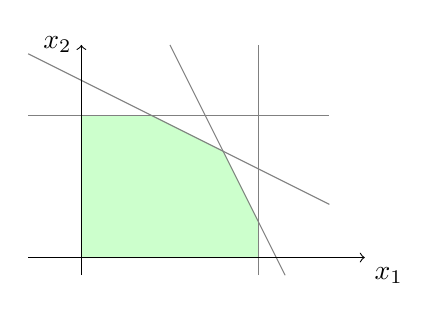
\begin{tikzpicture}[scale=.45]       
     
      \filldraw[fill=green!20,draw=green!20!](0,0) -- (0,4) -- (2,4) --
      (4,3) -- (5,1) -- (5,0) -- (0,0); 
      
      
      \draw [-,draw=gray] (7,1.5) -- (-1.5,5.75) ;
      \draw [-,draw=gray] (-1.5,4) -- (7,4) ;
      \draw [-,draw=gray] (5,-.5) -- (5,6) ;
      \draw [-,draw=gray] (2.5,6) -- (5.75,-.5) ;
      
      
          
      \draw[->] (-1.5,0) -- (8,0) node[below right] {$x_1$}; \draw[->]
      (0,-.5) -- (0,6) node[left] {$x_2$};
      
%      \draw[draw=blue] (-1.50000000000000,
%      7.40000000000000)node[left]{\small  
%        \color{blue}{$  \beta = 775$}} --
%      (8.37500000000000, -0.500000000000000) ; 
      
%      \filldraw [red] (4,3) circle (3pt)node[above right] {$(4,3)$};
      
          
%      \foreach \x in {1,...,7}
 %     \draw (\x cm,1pt) -- (\x cm,-1pt) node[anchor=north] {$\x$};
 %     \foreach \y in {1,...,5}
 %     \draw (1pt,\y cm) -- (-1pt,\y cm) node[anchor=east] {$\y$};     
    \end{tikzpicture} 
      \caption{The polyhedron of feasible solutions of the linear program \eqref{eq:1-4}.}
      \label{fig:1}
    \end{figure}

\end{example}








\begin{definition}
  \label{conv:def:2}
  A set $K\subseteq\setR^n$ is \emph{convex} if for each $u,v \in K$
  and $\lambda \in [0,1]$ the point $\lambda u+(1-\lambda)v$ is also
  contained in $K$. \end{definition}
\begin{figure}[htbp]
  \centering
  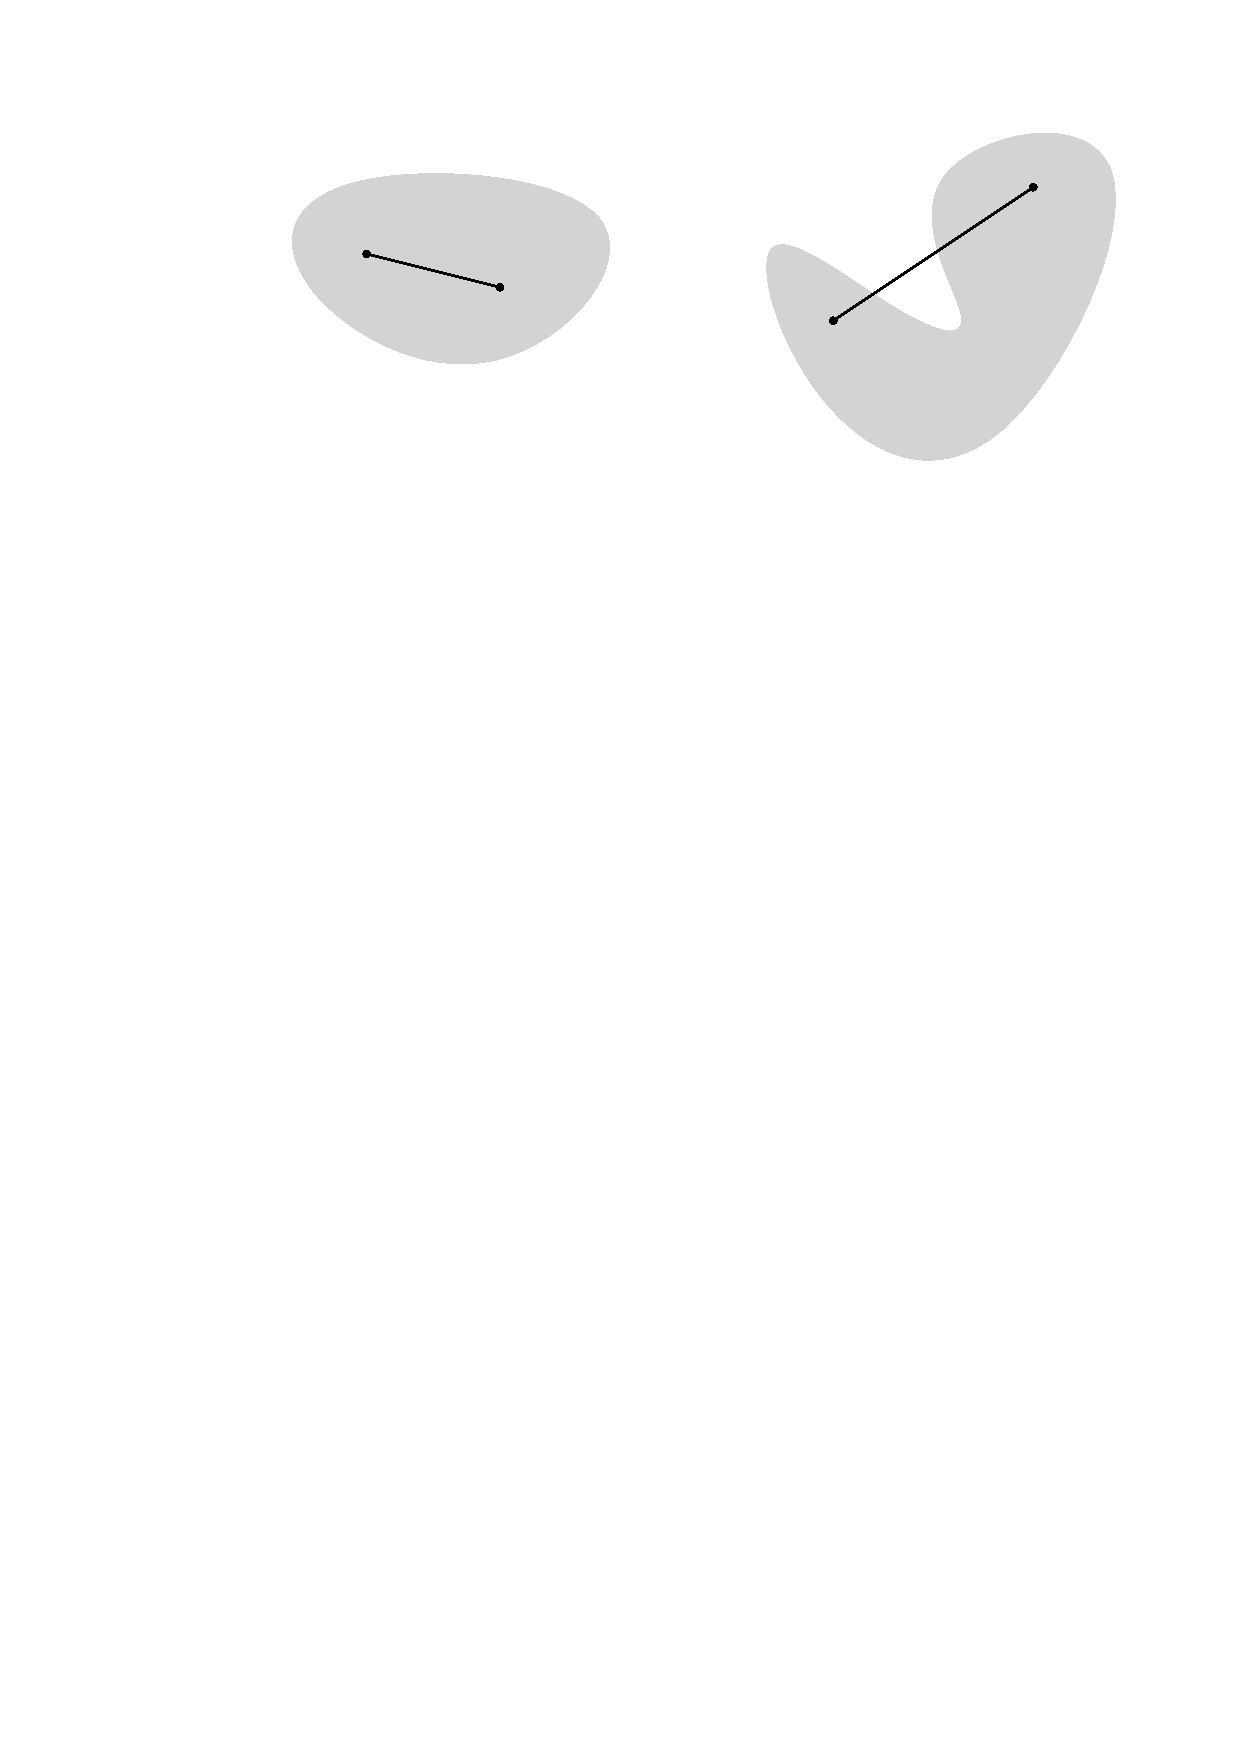
\includegraphics[height=3cm]{figures/exconv.pdf} 
  \caption{The set on the left is convex, the set on the right is  non-convex.}\label{conv:fig:3}
  
\end{figure}


A \emph{halfspace} is a set of solutions of one inequality $a^Tx \leq
\beta$ where $a \in \R^n$ and $\beta \in \R$, i.e., a set of the form
\begin{displaymath}
  \{ x \in \R^n \colon a^Tx \leq \beta\}. 
\end{displaymath} 
A \emph{hyperplane} is a set of the form 
\begin{displaymath}
  \{ x \in \R^n \colon a^Tx = \beta\}. 
\end{displaymath} 
It is easy to see that a halfspace is convex. Convexity is also maintained if convex sets are intersected. 

\begin{proposition}
  \label{lem:1}
  Let $I$ be an index set and $C_i \subseteq \R^n$ be convex sets for
  each $i \in I$, then $\cap_{i \in I}C_i$ is a convex set.
\end{proposition}

Consequently, the set of feasible solutions of a linear program $\{x
\in \R^n \colon Ax \leq b\}$ is a convex set. This is our motivation
to study properties of convex sets.


\section{Extreme points and vertices}
\label{sec:extr-points-vert}


\begin{definition}
  An inequality $a^Tx \leq \beta$ is \emph{valid} for a  set $K \subseteq \R^n$ if each $x^* \in K$ satisfies $a^Tx^* \leq \beta$.  If in addition $(c^Tx = \delta) \cap K \neq\emptyset$,
then $c^Tx\leq\delta$ is a \emph{supporting inequality} and $c^Tx = \delta$ is a
\emph{supporting hyperplane}. 
\end{definition}



% \begin{figure}
%   \centering  
%  \begin{tikzpicture}[scale=.45]       
     
%       \filldraw[fill=green!20,draw=green!20!](0,0) -- (0,4) -- (2,4) --
%       (4,3) -- (5,1) -- (5,0) -- (0,0); 
      
      
%       \draw [-,draw=gray] (7,1.5) -- (-1.5,5.75) ;
%       \draw [-,draw=gray] (-1.5,4) -- (7,4) ;
%       \draw [-,draw=gray] (5,-.5) -- (5,6) ;
%       \draw [-,draw=gray] (2.5,6) -- (5.75,-.5) ;
      
      
          
%       \draw[->] (-1.5,0) -- (8,0) node[below right] {$x_1$}; \draw[->]
%       (0,-.5) -- (0,6) node[left] {$x_2$};
% %\uncover<2->
% {      
%       \draw[draw=blue] (-1.50000000000000,
%       7.40000000000000)node[above]{\scriptsize  
%         \color{blue}{$  100 \cdot x_1 + 125 \cdot x_2 \leq 775$}} -- 
%       (8.37500000000000, -0.500000000000000) ; 
%       }
% % \uncover<5->
% {
      
% %       \filldraw [red] (4,3) circle (3pt)node[above right] {\scriptsize
% %         $(4,3)$};
%        }
          
% %      \foreach \x in {1,...,7}
%  %     \draw (\x cm,1pt) -- (\x cm,-1pt) node[anchor=north] {$\x$};
%  %     \foreach \y in {1,...,5}
%  %     \draw (1pt,\y cm) -- (-1pt,\y cm) node[anchor=east] {$\y$};     
%     \end{tikzpicture} 
    
%   \caption{The inequality $100\cdot x_1 + 125 \cdot x_2$ is valid for the set of feasible solutions of the linear program~\eqref{eq:1-4}. }
%   \label{fig:6}
% \end{figure}



\begin{definition}
  Let $K \subseteq \R^n$ be a convex set. A point $x^* \in K$ is an 
 \emph{extreme point} or \emph{vertex} of $K$ if there exists a valid inequality $a^Tx \leq \beta$ of $K$ such that 
 \begin{displaymath}
   \{x^*\} = K \cap \{x \in \R^n \colon a^Tx = \beta\}.  
 \end{displaymath}
In other words, if $x^*$ is the only point of $K$ that satisfies the valid inequality with equality. 
\end{definition}

\begin{figure}
  \centering
  
\includegraphics[height=3cm]{figures/ExtremePoint.pdf} 
  \caption{An extreme point of a convex set.}
  \label{fig:5}
\end{figure}

We can now characterize the extreme points of polyhedra. In fact, there are only finitely many of them. 

\begin{theorem}
  \label{thr:1}
  Let $P = \{x \in \R^n \colon Ax \leq b\}$ be a polyhedron. A feasible point $x^*$ is an extreme point of $P$ if and only if there is a sub-system $A'x \leq b'$ of  $Ax \leq b$  such that
  \begin{enumerate}[i)]
  \item $x^*$ satisfies all inequalities of $A'x \leq b'$ with
    equality. \label{item:1}
  \item $A'$ has $n$ rows and $A'$ is non-singular. \label{item:2}
  \end{enumerate}  
\end{theorem}


\begin{proof}
  Let $A'x \leq b'$ be such a sub-system and consider the valid
  inequality $\mathbf{1}^T A' x \leq \mathbf{1}^T b'$.  Clearly $x^*$
  satisfies this inequality with equality. Any $y^* \in P$ that
  satisfies this inequality with equality must satisfy $A'x = b'$.
  Since $A'$ is non-singular, $x^*$ is the unique solution of $A'x =
  b'$ which means that $x^*$ is the unique point of $P$ that satisfies
  $\mathbf{1}^T A' x \leq \mathbf{1}^T b'$ with equality. 

  Assume now that there does not exist a sub-system $A'x \leq b'$ of
  $Ax \leq b$ with properties~\ref{item:1}) and \ref{item:2}). Denote
  the sub-system of inequalities that are satisfied by $x^*$ with
  equality by $\wt{A}x \leq \wt{b}$. Then $\rank(\wt{A}) < n$ and
  there exists a $d \neq 0 \in \R^n$ with $\wt{A}d = 0$. Consequently
  there exists an $\varepsilon >0$ such that $x^* \pm \varepsilon
  \cdot d \in P$.

  Clearly, any inequality that is satisfied by $x^*$ with equality and
  that is satisfied by $x^* \pm\varepsilon d$ is satisfied by $x^*
  \pm\varepsilon d$ with equality as well. This implies that $x^*$ is
  not an extreme point.
 
\end{proof}



The relevance of vertices for linear programming is reflected in the following theorem. 

\begin{theorem}
  \label{thr:2}
  If a linear program $\max\{c^Tx \colon x \in \R^n, \, Ax \leq b\}$
  is feasible and bounded and if $\rank(A) = n$, then the linear program has an optimal solution that is  an extreme point. 
\end{theorem}


\begin{proof}
  We use the following notation. If $x^*$ is a feasible solution then
  $A_{x^*} x \leq b_{x^*}$ is the subsystem of $Ax \leq b$ that is
  satisfied by $x^*$ with equality. The rank of $x^*$, $\rank(x^*)$ is
  the rank of $A_{x^*}$.  The following claim implies the assertion. 
  \begin{quote}
    If $x^*$ is feasible and $\rank(x^*) < n$, then there exists a
    $y^*$ with $c^T y^* \geq c^Tx^*$ and $\rank(y^*)>\rank(x^*)$.
  \end{quote}
  To prove this, let $d \neq 0 \in \R^n$ be a vector with $A_{x^*}d =
  0$.  We can assume $c^Td \geq 0$ by switching to $-d$ otherwise.

  If $c^Td >0$, then consider the points $x^* + \lambda d$ with
  $\lambda \geq 0$ and let $\lambda_{max}$ be maximal with the
  corresponding point feasible. Clearly $y^* = x^* + \lambda_{max} d$
  satisfies the condition of the claim. 

  Suppose now that  $c^T d = 0$. Then $A d \neq 0$ since $\rank(A) = n$. Let $\lambda_{max}$ be the maximum of the set $\{\lambda \geq 0 \colon A (x^* \pm \lambda d) \leq b\}$. Then $y^* = x^* + \lambda_{max}d$ or $y^* = x^* - \lambda_{max}d$  satisfies the condition of the claim. 
  
\end{proof}



\begin{corollary}
  \label{co:12}
  A linear program $\max \{ c^Tx : x ∈ ℝ^n, \, Ax ≤ b\}$ which is feasible and bounded has an optimal solution. 
\end{corollary}


\begin{proof}
  The linear program 
  \begin{displaymath}
    \max \{ c^Tx^+ -c^T x^- : x^+,x^- ∈ ℝ^n, x^+≥0, \, x^‐≥0, \, A(x^+-x^-) ≤ b\}
  \end{displaymath}
 is feasible and bounded and the rank of the constraint matrix is $2\,n$.  Thus, by Theorem~\ref{thr:2} possesses an optimal solution. $x^+,x^-$. This corresponds to an optimal solution $x^+-x^-$ of the linear program $\max \{ c^Tx : x ∈ ℝ^n, \, Ax ≤ b\}$. 
\end{proof}

\section{Linear, affine, conic  and convex hulls}
\label{conv:cha:linear-affine-convex}



We now describe convex sets that are generated by a set 
 $X\subseteq\setR^n$  of $n$-dimensional
vectors. The \emph{linear hull}, \emph{affine hull}, \emph{conic hull} and \emph{convex
  hull} of $X$ are defined as follows.
\begin{eqnarray}
  \linhull(X) & = & \{ \lambda_1 x_1+ \cdots + \lambda_t x_t \mid t\geq0,  \label{conv:eq:2}\\
   & & \quad \quad  x_1,\ldots,x_t
  \in  X, \, \lambda_1,\ldots,\lambda_t\in \setR\} \nonumber \\
  \affhull(X) & = & \{ \lambda_1 x_1+ \cdots + \lambda_t x_t \mid t\geq1, \label{conv:eq:4}\\
  & &   \quad \quad  x_1,\ldots,x_t \in  X, \, \sum_{i=1}^t \lambda_i = 1, \,
  \lambda_1,\ldots,\lambda_t\in \setR\} \nonumber   \\ 
  \cone(X)  & = & \{ \lambda_1 x_1+ \cdots + \lambda_t x_t \mid t\geq0, \label{conv:eq:5} \\
  &&     \quad \quad  x_1,\ldots,x_t \in  X,  \, \lambda_1,\ldots,\lambda_t\in
  \setR_{\geq0}\} \nonumber \\
  \conv(X) & = & \{ \lambda_1 x_1+ \cdots + \lambda_t x_t \mid t\geq1, \label{conv:eq:6} \\
  &&     \quad \quad  x_1,\ldots,x_t \in  X, \,  \sum_{i=1}^t \lambda_i = 1, \, \lambda_1,\ldots,\lambda_t\in
  \setR_{\geq0}\} \nonumber 
\end{eqnarray}



\begin{figure}[htbp]
  \begin{center}
    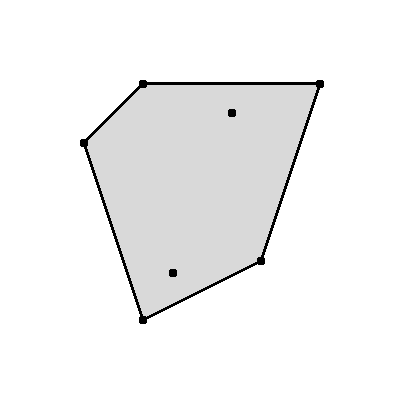
\includegraphics{figures/picture1.pdf}    
  \end{center}
  \caption{The convex hull of $7$ points in $\setR^2$. }\label{conv:fig:2}
\end{figure}


\begin{figure}[htbp]
  \begin{center}{
      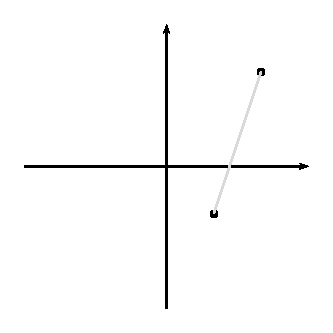
\includegraphics{figures/picture2-1.pdf} 
      \hfill
      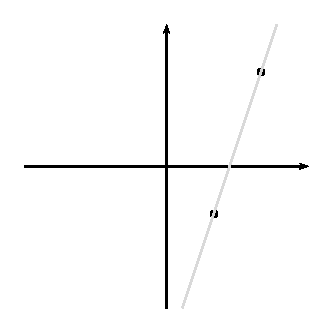
\includegraphics{figures/picture2-2.pdf} 
    }
    
  \end{center}
  \caption{Two points with their convex hull on the left and  their
    affine hull on the right. }\label{conv:fig:1}
\end{figure}





\begin{figure}[htbp]
  \begin{center}{
   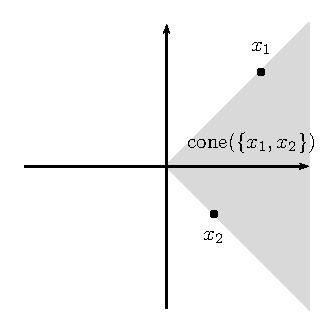
\includegraphics{figures/picture3.pdf}

    }
    
  \end{center}
  \caption{Two points with their conic hull}\label{conv:fig:4}
\end{figure}



\begin{proposition}
  \label{conv:prop:1}
  Let $X\subseteq\setR^n$ and $x_0\in X$. One has 
  \begin{displaymath}
    \affhull(X) = x_0 + \linhull(X - x_0),
  \end{displaymath}
  where for $u \in \setR^n$ and $V\subseteq\setR^n$,   $u +V$ denotes the set
  $u+V = \{ u+v \mid v \in V\}$.
\end{proposition}


\begin{proof}
  We first show that each $x \in \affhull(X)$ is also an element of the
  set $ x_0 + \linhull(X-x_0)$ and then we show that each point $x \in
  x_0 + \linhull(X-x_0)$ is also an element of $\affhull(X)$.


  Let $x \in \affhull(X)$,i.e., there exists a natural number $t\geq1$
  and $\lambda_1,\ldots,\lambda_t \in \setR$, with $x = \lambda_1x_1+\cdots+\lambda_t x_t$ and
  $\sum_{i=1}^t\lambda_i=1$. Now
  \begin{eqnarray*}
    x & = &  x_0  - x_0 + \lambda_1 x_1+   \lambda_2x_2+\cdots+\lambda_t x_t \\
    & = & x_0  - \lambda_1x_0 -  \cdots-\lambda_t x_0 + \lambda_1 x_1+  \lambda_2x_2+\cdots+\lambda_t x_t \\
    & = & x_0 +\lambda_1(x_1-x_0)+\cdots+\lambda_t (x_t-x_0),
  \end{eqnarray*}
  which shows that $x \in x_0 + \linhull(X - x_0)$. 


  Suppose now that
  $x \in x_0 + \linhull(X - x_0)$. Then there exist $\lambda_1,\ldots,\lambda_t\in \setR$
  with $x = x_0 +\lambda_1(x_1-x_0)+\cdots+\lambda_t (x_t-x_0)$. With $\lambda_0 = 1
  -\sum_{i=1}^t \lambda_i$ one has $\sum_{i=0}^t \lambda_i =1$ and
  \begin{eqnarray*}
    x & = &  x_0 +\lambda_1(x_1-x_0)+\cdots+\lambda_t (x_t-x_0)\\
    & = & \lambda_0 x_0 + \cdots + \lambda_t x_t
  \end{eqnarray*}
  and thus that $x \in \affhull(X)$.  \qed 

\end{proof}






\begin{theorem}
  \label{conv:thr:1}
  Let $X\subseteq\setR^n$ be a set of points. The convex hull, $\conv(X)$,  of $X$
  is convex. 
\end{theorem}

\begin{proof}
  Let $u$ and $v$ be points in $\conv(X)$. This means that there exists
  a natural number $t\geq1$,  real numbers  $\alpha_i,\beta_i\geq0$, and points $x_i
  \in X$,  $i=1,\ldots,t$ with
  $\sum_{i=1}^t \alpha_i = \sum_{i=1}^t \beta_i =1$ with  $u =  \sum_{i=1}^t
  \alpha_ix_i$  and $v = \sum_{i=1}^t \beta_ix_i$. For $\lambda \in [0,1]$ one has 
  $\lambda\alpha_i+(1-\lambda)\beta_i\geq0$ for $i=1,\ldots,t$  and $\sum_{i=1}^t
  \left(\lambda\alpha_i+(1-\lambda)\beta_i \right) =1$. This shows that   
  \begin{displaymath}
    \lambda u + (1-\lambda) v  =  \sum \left(\lambda_i \alpha_i + (1- \lambda_i) \beta_i\right)
    x_i  \in \conv(X),
  \end{displaymath}
  and therefore that $\conv(X)$ is convex. 
\qed \end{proof}

\begin{theorem}
  \label{conv:thr:2}
  Let $X\subseteq\setR^n$ be a set of points. Each convex set $K$ containing $X$
  also contains $\conv(X)$. 
\end{theorem}

\begin{proof}
  Let $K$ be a convex set containing $X$, 
  and let $x_1,\ldots,x_t\in X$ and $\lambda_i\in \setR$ with $\lambda_i\geq0$, $i=1,\ldots,t$ and
  $\sum_{i=1}^t  \lambda_i =1$. We need to show that $u = \sum_{i=1}^t \lambda_i
  x_i$ is contained in  $K$.   This is true for $t\leq2$ by the definition
  of convex sets.  

  We argue by induction.  Suppose that $t\geq3$. If one of the $\lambda_i$ is
  equal   to $0$, then one can represent $u$ as a convex combination
  of $t-1$ points in $X$ and, by induction, $u \in K$. If    $t\geq3$,
  each $\lambda_i>0$ and $\sum_{i=1}^t \lambda_i = 1$, then one has $0<\lambda_i<1$ for
  $i=1,\ldots,t$ and thus we can write 
  \begin{displaymath}
    u = \lambda_1 x_1 + (1-\lambda_1) \sum_{i=2}^t \frac{\lambda_i}{1-\lambda_1} x_i. 
  \end{displaymath}
  One has $\lambda_i / (1-\lambda_1)>0$ and 
  \begin{displaymath}
    \sum_{i=2}^t \frac{\lambda_i}{1-\lambda_1} = 1,
  \end{displaymath}
  which means that the point $\sum_{i=2}^t \frac{\lambda_i}{1-\lambda_1} x_i$ is in
  $K$ by induction. Again, by the definition of convex sets, we
  conclude that $u$ lies in $K$. 
\qed \end{proof}

Theorem~\ref{conv:thr:2} implies that $\conv(X)$ is the intersection of all
convex sets containing $X$, i.e., 
\begin{displaymath}
  \conv(X) = \bigcap_{\substack{K \supseteq X\\ K \text{  convex}}} K. 
\end{displaymath}



\begin{definition}
  \label{conv:def:4}
  A set $C\subseteq\setR^n$ is a \emph{cone}, if it is convex and for each $c \in
  C$ and each $\lambda \in \setR_{\geq0}$ one has  $\lambda\cdot c \in C$. 
\end{definition}

Similarly to Theorem~\ref{conv:thr:1} and Theorem~\ref{conv:thr:2} one proves
the following. 
\begin{theorem}
  \label{conv:thr:8}
  For any $X\subseteq\setR^n$, the set $\cone(X)$ is a cone. 
\end{theorem}

\begin{theorem}
  \label{conv:thr:9}
  Let $X\subseteq\setR^n$ be a set of points. Each cone containing $X$ also
  contains $\cone(X)$. 
\end{theorem}

These theorems imply that $\cone(X)$ is the intersection of all
cones  containing $X$, i.e., 
\begin{displaymath}
  \cone(X) = \bigcap_{\substack{C \supseteq X\\ C \text{  is a cone}}} C. 
\end{displaymath}


\section{Radon's lemma and Carath\'eodory's theorem}
\label{conv:sec:radons-lemma-carath}

\begin{theorem}[Radon's lemma]
  \label{conv:thr:6}
  Let $A\subseteq\setR^n$ be  a set of $n+2$ points. There exist disjoint
  subsets $A_1,A_2\subseteq A$ with
  \begin{displaymath}
    \conv(A_1) \cap \conv(A_2) \neq \emptyset.
  \end{displaymath}
\end{theorem}

\begin{proof}
  Let $A = \{a_1,\ldots,a_{n+2}\}$. We embed these points into $\setR^{n+1}$
  by appending a $1$ in the $n+1$-st component, i.e., we construct 
  \begin{displaymath}
    A' = \left \{ \smat{a_1\\1}, \ldots,\smat{a_{n+2}\\1} \right\}\subseteq\setR^{n+1}.
  \end{displaymath}
  The set $A'$ consists of $n+2$ vectors in $\setR^{n+1}$. Those vectors
  are linearly dependent.  Let 
  \begin{equation}
    \label{conv:eq:1}
    0= \sum_{i=1}^{n+2} \lambda_i \smat{a_i\\1}
  \end{equation}
  be  a nontrivial linear representation of  $0$, i.e., not all $\lambda_i$
  are~$0$.  Furthermore, let $P = \{i \colon \lambda_i \geq0, \, i=1,\ldots,n+2\}$
  and $N = \{i   \colon \lambda_i <0, \, i=1,\ldots,n+2\}$. We claim that
  \begin{displaymath}
      \conv(\{a_i \colon i \in P\}) \cap \conv(\{a_i  \colon i \in N\} ) \neq \emptyset.
  \end{displaymath}
  It follows from~\eqref{conv:eq:1} and the fact that the $n+1$-st
  component of the vectors is $1$  that $\sum_{i \in P} \lambda_i = - \sum_{i \in N}
  \lambda_i  = s >0$. It follows also from~\eqref{conv:eq:1} that 
  \begin{displaymath}
     \sum_{i \in P} \lambda_i a_i = \sum_{i \in N} -\lambda_i a_i.
  \end{displaymath}
  The point $ u = \sum_{i \in P} (\lambda_i / s) \cdot  a_i  = \sum_{i \in N} (-\lambda_i
  /s) a_i $ is contained in $ \conv(\{a_i \colon i \in P\}) \cap \conv(\{a_i
  \colon i \in N\} )$, implying the claim.  \qed
  
\end{proof}


\begin{theorem}[Carath\'eodory's theorem]
  \label{conv:thr:7}
  Let $X\subseteq\setR^n$, then for each $x \in \cone(X)$ there exists a set
  $\wt{X}\subseteq X$ of cardinality at most $n$  such that $x \in
  \cone(\wt{X})$. The vectors in $\wt{X}$ are linearly independent. 
\end{theorem}


\begin{proof}
  Let $x \in \cone(X)$, then there exist $t \in \setN_+$, $x_i \in X$ and
  $\lambda_i\geq0$, $i=1,\ldots,t$, with  $ x = \sum_{i=1}^t \lambda_i x_i$.
  Suppose that $t\in \setN_+$ is minimal such that $x$ can be represented
  as   above. We claim that $t \leq n$. If $t\geq n+1$, then the $x_i$ are
  linearly dependent.  This means that there are $\mu_i \in \setR$, not all
  equal to $0$ with   
  \begin{equation}
    \label{conv:eq:13}
    \sum_{i=1}^t \mu_i x_i = 0.
  \end{equation}
 By multiplying each
  $\mu_i$ in \eqref{conv:eq:13} with   $-1$ if necessary, we can  assume
  that at least one of the  $\mu_i$ is strictly larger than $0$.  
  One
  has for each $\varepsilon \in \setR$  
  \begin{equation}
    \label{conv:eq:14}
    x = \sum_{i=1}^t (\lambda_i - \varepsilon \cdot \mu_i) x_i. 
  \end{equation}
  What is the largest $\varepsilon^*>0$ that we can pick for $\varepsilon$ such
  that~\eqref{conv:eq:14} is still a conic combination? We need to have
  \begin{equation}
    \label{conv:eq:15}
      \lambda_i - \varepsilon \cdot \mu_i \geq0, \,\text{  for each }i \in \{1,\ldots,t\}. 
  \end{equation} 
   Let $J$ be the set of indices $J = \{j  \colon j \in \{1,\ldots,t\}, \, \mu_j
   >0\}$. We observed that we can assume $J \neq \emptyset$. 
We have~\eqref{conv:eq:15} as long as 
  \begin{equation}
    \label{conv:eq:16}
    \varepsilon \leq  \lambda_j / \mu_j \text{ for each } j \in J.
  \end{equation}
This means that $\varepsilon^* = \min\{ \lambda_j / \mu_j \colon j \in J\}$.  Let $j^*\in J$
be an index where this minimum is attained.  
Since $\lambda_i - \varepsilon^* \cdot \mu_i \geq0$ for all $i=1,\ldots,t$ and since
$\lambda_{j^*}-\varepsilon^*\cdot\mu_{j^*}=0$, we have $x \in  \cone(\{x_1,\ldots,x_t\}\setminus
\{x_{j^*}\}$, which is a contradiction to the minimality of~$t$.
\qed
\end{proof}


\begin{corollary}[Carath\'eodory's theorem for convex hulls]
  \label{conv:co:1}
  Let $X\subseteq\setR^n$, then for each $x \in \conv(X)$ there exists a set
  $\wt{X}\subseteq X$ of cardinality at most $n+1$ such that $x \in
  \conv(\wt{X})$. 
\end{corollary}




\section{Separation theorem and Farkas' lemma}
\label{conv:sec:separ-theor-fark}


We recall a basic fact from analysis, see,
e.g.~\cite[Theorem~4.4.1]{MarsdenHoffman93}. 

\begin{theorem}
  \label{conv:thr:11}
  Let $X\subseteq\setR^n$ be compact and $f: X \to \setR$ be continuous. Then $f$ is
  bounded and there exist
  points $x_1,x_2 \in X$ with $f(x_1) = \sup\{ f(x) \colon  x \in X\}$ and
  $f(x_2) = \inf \{ f(x) \colon x \in X\}$. 
\end{theorem}


\begin{theorem}
  \label{conv:thr:10}
  Let $K\subseteq\setR^n$ be a closed  convex set and $x^* \in \setR^n \setminus K$, then there
  exists an inequality $a^Tx\geq\beta$ such that $a^T y > \beta$ holds for all
  $y \in K$ and $a^Tx^*<\beta$. 
\end{theorem}

\begin{proof}
  Since the mapping $f(x) = \|x^*-x\|$ is continuous and since for any
  $k \in K$, $K \cap \{ x \in K \colon \|x^* - x\|\leq \|x^* - k\|\}$ is
  compact, there exists a point $k^* \in K$ with minimal distance to
  $x^*$. Consider the midpoint $m = 1/2(k^*+x^*)$ on the line-segment
  $\overline{k^*x^*}$   and the hyperplane $a^Tx = \beta$ with $\beta = a^Tm$ and $a =
  (k^*-x^*)$. Clearly, $a^T x^* = \beta - 1/2 \|k^*-x^*\|^2$ and $a^T k^*
  = \beta +  1/2 \|k^*-x^*\|^2$. Suppose that there exists a $k' \in K$
  with $a^T k' \leq \beta$. The points $\lambda k^* + (1-\lambda) k', \,\lambda \in [0,1]$ are in 
  $K$ by the convexity of $K$, thus we can also assume that $k'$ lies
  on the hyperplane, i.e., $a^Tk' = \beta$. This means that there exists
  a vector $x'$ which is orthogonal to $a$   and $k' = m +
  x'$. The distance squared  of a point $\lambda k^* + (1-\lambda) k'$  with $\lambda \in [0,1]$
  to $m$  is, by Pythagoras equal to 
  \begin{displaymath}
    \lambda^2  \|\frac{1}{2} a\|^2 + (1-\lambda)^2 \|x'\|^2.
  \end{displaymath}
  As a function of $\lambda$, this is increasing 
  at $\lambda=1$. Thus there exists a point on the line-segment $\lambda x^* +
  (1-\lambda) k'$  which is closer to $m$ than $k^*$. This point is also
  closer to $x^*$ than $k^*$, which is a contradiction.  Therefore
  $a^Tk >\beta$ for each $k \in K$. 
  \qed 
\end{proof}


\begin{theorem}[Farkas' lemma]
  \label{conv:thr:12}
  Let $A \in \setR^{m\times n}$ be a matrix and $b \in \setR^m$ be a vector. The
  system $Ax = b, \,x\geq0$ has a solution if and only if for all $\lambda \in
  \setR^m$ with $\lambda^TA\geq0$ one has $\lambda^Tb \geq0$.  
\end{theorem}

\begin{proof}
  Suppose that $x^* \in \setR^n_{\geq0}$ satisfies $Ax^* = b$ and let $\lambda \in
  \setR^m$ with $\lambda^T A \geq0$. Then $\lambda^Tb = \lambda^TA x^* \geq0$, since
  $\lambda^TA\geq0$ and $x^*\geq0$. 

  Now suppose that $Ax = b, \,x\geq0$ does not have a solution. Then,
  with   $X\subseteq\setR^n$ being  the set of column vectors of $A$, 
  $b$ is not in $\cone(X)$. The set $\cone(X)$ is convex and
  closed, see exercise~\ref{conv:item:2}. Theorem~\ref{conv:thr:10} implies 
  that there is an inequality $\lambda^Tx \geq \beta$ such that $\lambda^Ty > \beta$ for
  each $y \in \cone(X)$ and $\lambda^Tb < \beta$. Since for each $a \in X$ and
  each $\mu\geq0$ one has $\mu\cdot a \in \cone(X)$  and thus  $\lambda^T (\mu\cdot a)
  >\beta$, it follows that $\lambda^T a \geq0$ for each $a \in X$. Furthermore,
  since $0 \in \cone(X)$ it follows that $0\geq\beta$ and thus that
  $\lambda^Tb<0$. 
  
\end{proof}

\section{Decomposition theorem for polyhedra}
\label{sec:decomp-theor-polyh}

In the following we use the notation $P(A,b) = \{x \in\R^n \colon Ax \leq b\}$ for the polyhedron that is defined by $Ax \leq b$. We prove the Minkowski-Weyl theorem in this section that shows that polyhedra can be decomposed into the Minkowski sum of a polytope and a cone. 

\begin{definition}
\label{po:def:5}
An inequality $a^Tx\leq\beta$ is called an \emph{implicit equality} of
$Ax\leq b$ if each $x^* \in P(A,b)$ satisfies $a^Tx^* = \beta$. We denote the
subsystem  consisting of implicit equalities of $Ax\leq b$ by $A^=x\leq b^=$
and the subsystem consisting of the other inequalities by
$A^\leq x\leq b^\leq$. A constraint is \emph{redundant} if its removal from
$Ax\leq b$ does not change the set of feasible solution of $Ax\leq b$.  
\end{definition}

In the following, a vector $x$ satisfies $Ax < b$ if and only if
$a_i^T x < b_i$ for all $1\leq i\leq m$, where $a_1$,\ldots,$a_m$ are the rows of $A$.

\begin{lemma}
  \label{po:lem:3}
  Let $P(A,b)$ be a non-empty polyhedron.
  Then there exists an $x \in P(A,b)$ with $A^\leq x<b^\leq$. 
\end{lemma}
\begin{proof}
  Suppose that the inequalities in  $A^\leq x\leq b^\leq$ are $a_1^Tx\leq\beta_1
  ,\ldots,a_k^Tx\leq\beta_k$. For each $1\leq i\leq k$ there exists an $x_i \in P$ with
  $a_i^Tx_i<\beta_i$. Thus the point $x = 1/k (x_1+\cdots+x_k)$ is a point of
  $P(A,b)$ satisfying  $A^\leq x<b^\leq$. 
\end{proof}


\begin{lemma}
  \label{po:lem:2}
  Let $Ax\leq b$ be a system of inequalities. One has 
  \begin{displaymath}
    \affhull(P(A,b)) = \{ x \in \setR^n \mid A^=x = b^=\} = \{ x \in \setR^n \mid A^=x\leq b^=\}.
  \end{displaymath}
\end{lemma}
\begin{proof}
  Let $x_1,\ldots,x_t \in P(A,b)$ and suppose that $a^Tx\leq\beta$ is an
  implicit equality. Then since $a^Tx_i = \beta$ one has
  $a^T(\sum_{j=1}^t\lambda_ix_i) = \beta$. Therefore the inclusions $\subseteq$
  follow. 

  Suppose now that $x_0$ satisfies $A^=x\leq b^=$. Let $x_1 \in P(A,b)$
  with $A^\leq x_1<b^\leq$. If $x_0=x_1$ then $x_0 \in P(A,b) \subseteq
  \affhull(P(A,b))$.  Otherwise the line segment between $x_0$ and
  $x_1$ contains more than one point in $P$ and thus $x_0 \in
  \affhull(P)$. 
\end{proof}








A nonempty set  $C\subseteq\setR^n$ is a \emph{cone} if $\lambda\, x + \mu\,y \in C$
for each $x,y\in C$ and $\lambda,\mu\in \setR_{\geq0}$. A cone  $C$ is \emph{polyhedral}
if $C = \{ x \in \setR^n \mid Ax\leq0\}$. A cone \emph{generated by} vectors
$x_1,\ldots,x_m \in \setR^n$ is a set of the form $C = \{ \sum_{i=1}^m \lambda_i x_i
\mid \lambda_i\in \setR_{\geq0}, \, i=1,\ldots,m\}$.   A point $x = \sum_{i=1}^m \lambda_i x_i$
with  $\lambda_i\in \setR_{\geq0}, \, i=1,\ldots,m$ is called a \emph{conic
  combination}   of the $x_1,\ldots,x_m$. The set of conic combinations of
$X$ is denoted by $\cone(X)$. 


\begin{theorem}[Farkas-Minkowsi-Weyl theorem]
  \label{po:thr:3}
  A convex cone is polyhedral if and only if it is finitely
  generated. 
\end{theorem}


\begin{proof}
  Suppose that $a_1,\ldots,a_m$ span $\setR^n$ and consider the cone $C = \{
  \sum_{i=1}^m \lambda_i a_i \mid \lambda_i\geq0, \, i=1,\ldots,m\}$.
  Let $b \notin C$.
  Then the system $A\lambda = b$, $\lambda \geq 0$ has no solution.
  By Theorem~\ref{conv:thr:12} (Farkas' lemma), this implies that there exists a $y\in\setR^n$
  such that $A^Ty \leq 0$ and $b^Ty > 0$.

  Suppose that the columns of $A$ which correspond to
  inequalities in $A^Ty\leq0$   that are satisfied  by $y$ with equality
  have rank $<n-1$.
  Denote these columns by $a_{i_1},\ldots,a_{i_k}$.  
  Then there exists a $v\neq0$ which is orthogonal to
  each of these columns and to $b$, i.e., $a_{i_j}^Tv = 0$ for each
  $j=1,\ldots,k$ and $b^Tv =0 $. 
  There also exists a column $a^*$ of $A$ which is not in the set
  $\{a_{i_1},\ldots,a_{i_k}\}$ such that $(a^*)^Tv>0$ since the columns of
  $A$ span $\setR^n$. Therefore there exists an $\epsilon>0$ such that 
  \begin{enumerate}[i)]
  \item $A^T(y + \epsilon \cdot v)\leq0$ 
  \item The subspace generated by the columns of $A$ which correspond
    to inequalities of $A^Tx\leq0$ which are satisfied by $y + \epsilon \cdot v$
    with equality strictly contains $\langle a_{i_1},\ldots,a_{i_k}\rangle$. 
  \end{enumerate}
  
  Notice that we have $b^Ty = b^T(y + \epsilon \cdot v)>0$. 

  Continuing this way, we obtain a solution of the form $y + u$ of
  $A^Tx\leq0$ such that one has $n-1$ linearly independent columns of $A$
  whose corresponding inequality in $A^Tx\leq0$ are satisfied with
  equality.   Thus we see that each $b$ which does
  not belong to $C$ can be separated from $C$ with an inequality of
  the form $c^Tx\leq0$  which
  is uniquely defined by $n-1$ linearly independent vectors from the set
  $a_1,\ldots,a_m$.  This shows that $C$ is polyhedral. 

  Suppose now that $a_1,\ldots,a_m$ do not span $\setR^n$. Then there  exist
  linearly independent vectors $d_1,\ldots,d_k$ such that each $d_i$ is
  orthogonal to each of the $a_1,\ldots,a_m$ and $a_1,\ldots,a_m,d_1,\ldots,d_k$
  spans $\setR^n$.   The cone generated by
  $a_1,\ldots,a_m,d_1,\ldots,d_k$ is polyhedral and thus of the form $Ax\leq0$
  with some matrix $A\in \setR^{m\times n}$. Suppose that  $\langle a_1,\ldots,a_m\rangle = \{x
  \in \setR^n \mid Ux = 0\}$.  Now $C = \{ x \in \setR^n \mid Ax\leq0, \, Ux = 0\}$
  and $C$ is polyhedral. 


  Now suppose that $C = \{ x \in \setR^n \mid a_1^Tx\leq0,\ldots,a_m^Tx\leq0\}$.
  The cone
  \[ C' := \cone(a_1,\ldots,a_m) = \{ \sum_{i=1}^m \lambda_i a_i \mid
  \lambda_i\geq0,\,i=1,\ldots,m\} \]
  is polyhedral and thus of the form $C' = \{ x
  \in \setR^n \mid b_1^Tx\leq0, \ldots,b_k^Tx\leq0\}$. Clearly,
  $\cone(b_1,\ldots,b_k)\subseteq C$  since $b_i^Ta_j\leq0$. Suppose now that $y \in
  C \textbackslash{} \cone(b_1,\ldots,b_k)$. Then, since $\cone(b_1,\ldots,b_k)$ is
  polyhedral, there exists a $w\in \setR^n$ with $w^Ty>0$ and $w^Tb_i\leq0$
  for each $i=1,\ldots,k$. From the latter we conclude that $w \in
  C'$. From $y \in C$ and $w \in C'$ we conclude $w^Ty\leq0$, which is a contradiction.
\end{proof}

A set of vectors $Q = \conv(X)$, where $X\subseteq\setR^n$ is finite is called a
\emph{polytope}. 

\begin{theorem}[Decomposition theorem for polyhedra]
  \label{po:thr:4}
  A set $P\subseteq\setR^n$ is a polyhedron if and only if $P = Q + C$ for some
  polytope $Q$ and a polyhedral cone $C$. 
\end{theorem}

\begin{proof}
  Suppose $P = \{ x \in \setR^n \mid Ax\leq b\}$ is a polyhedron. Consider the
  polyhedral cone 
  \begin{equation}
    \label{po:eq:6}
    \left\{\mat{x\\\lambda} \mid x \in \setR^n, \, \lambda \in \setR_{\geq0}; Ax -
      \lambda b\leq0\right\} 
  \end{equation}
  is generated by finitely many vectors $\mat{x_i\\\lambda_i}$,
  $i=1,\ldots,m$. By scaling with a positive number we may assume that
  each $\lambda_i\in \{0,1\}$.  Let $Q$ be the convex hull of the $x_i$ with
  $\lambda_i=1$ and let $C$ be the cone generated by the $x_i$ with
  $\lambda_i=0$. A point $x \in \setR^n$ is in $P$ if and only if $\mat{x\\1}$
  belongs to~\eqref{po:eq:6} and thus if and only if 
  \begin{displaymath}
    \mat{x\\1} \in
    \cone\left\{\mat{x_1\\\lambda_1},\ldots,\mat{x_m\\\lambda_m}\right\}. 
  \end{displaymath}
  Therefore $P = Q + C$. 


  Suppose now that $P = Q+C$ for some polytope $Q$ and a polyhedral
  cone $C$ with $Q = \conv(x_1,\ldots,x_m)$ and $C = \cone(y_1,\ldots,y_t)$. A
  vector $x_0$ is in $P$ if and only if 
  \begin{equation}
    \label{po:eq:7}
    \mat{x_0\\1} \in \cone\left\{\mat{x_1\\1},\ldots, \mat{x_m\\1},\mat{y_1\\0},\ldots,\mat{y_t\\0}     \right\}
  \end{equation}
By Theorem~\ref{po:thr:3} \eqref{po:eq:7} is equal to 
\begin{equation}
\label{po:eq:12}
  \left\{ \mat{x\\\lambda} \mid Ax - \lambda b \leq0\right\}
  \end{equation}
for some matrix $A$ and vector $b$.  Thus $x_0\in P$  if and only if
$Ax_0\leq b$ and thus $P$ is a polyhedron.

\end{proof}




\begin{figure}[htbp]
  \begin{center}
    %\resizebox{4cm}{4cm}
  \end{center}
  \caption{A polyhedron and its decomposition into $Q$ and $C$\label{po:fig:decomp}}
\end{figure}




Let $P = \{ x \in \setR^n \mid Ax\leq b\}$. The \emph{characteristic cone} is 
$\charcone(P) =\{ y \mid y+x \in P \text{ for all } x \in P\} = \{y \mid Ay
\leq0\}$. One has
\begin{enumerate}[i)]
\item $y \in \charcone(P)$ if and only if there exists an $x \in P$ such
  that $x + \lambda\,y \in P$ for all $\lambda\geq0$ 
\item $P + \charcone(P)=P$
\item $P$ is bounded if and only if $\charcone(P)=\{0\}$. 
\item If the decomposition of $P$ is $P = Q +C$, then $C = \charcone(P)$. 
\end{enumerate}



The \emph{lineality space} of $P$ is defined as $\charcone(P) \cap -
\charcone(P)$. A polyhedron is \emph{pointed}, if its lineality space is
$\{0\}$.






%\subsection{Faces}
%\label{po:sec:faces}
\begin{definition}
  \label{def:f4}
  A set $F\subseteq\setR^n$ is called a \emph{face} of $P$ if there exists a
  valid inequality $c^Tx\leq\delta$ for $P$ with $F = P \cap (c^Tx = \delta)$. 
\end{definition}
 
\begin{lemma}
  \label{po:lem:4}
  A set $\emptyset \neq F \subseteq \setR^n$ is a face of $P$
  if and only if $F = \{ x \in P \mid A'x = b'\}$ for a subset $A'x\leq b'$ of $Ax\leq b$.
\end{lemma}

\begin{proof}
  Suppose that $F = \{ x \in P \mid A'x = b'\}$. Consider the vector $c =
  1^TA'$ and $\delta = 1^Tb'$. The inequality $c^Tx\leq \delta$ is valid for
  $P$. It is satisfied with equality by each $x \in F$. If $x' \in P\textbackslash{}
  F$, then there exists an inequality $a^Tx\leq\beta$ of $A'x\leq b'$ such
  that $ a^Tx' < \beta$ and consequently $c^Tx'<\delta$. 

  On the other hand, if $c^Tx\leq\delta$ defines the face $F$,
  then by the linear programming duality (see chapter~\ref{cha:duality})
  \[ \max\{ c^Tx \mid Ax\leq b \} = \min\{ b^T\lambda \mid A^T\lambda = c, \lambda \geq 0 \} \]
  there exists a $\lambda \in \setR^m_{\geq 0}$ such that $c=\lambda^TA$ and $\delta = \lambda^Tb$.
  Let $A'x\leq b'$ be the
  subsystem of $Ax\leq b$ which corresponds to strictly positive entries
  in $Ax\leq b$. One has $F = \{ x \in P \mid A'x = b'\}$. 
\end{proof}





A \emph{facet} of $P$ is an inclusion-wise maximal face $F$ of $P$
with $F\neq P$.  An inequality $a^Tx\leq\beta$ of $Ax\leq b$ is called
\emph{redundant} if $P(A,b) = P(A',b')$, where $A'x\leq b'$ is the system
stemming from $Ax\leq b$ by deleting $a^Tx\leq\beta$.  A system $Ax\leq b$ is
irredundant if $Ax\leq b$ does not contain a redundant inequality.

\begin{lemma}
  \label{po:lem:1}
  Let $Ax\leq b$ be an irredundant system. 
  Then a set $F\subseteq P$ is a facet if and only if it is
  of the form $F = \{ x \in P \mid a^Tx = \beta\}$ for an
  inequality $a^Tx\leq\beta$ of $A^\leq x\leq b^\leq$. 
\end{lemma}


\begin{proof}
  Let $F$ be a facet of $P$. Then $F = \{x \in P \mid c^Tx\leq\delta\}$ for a valid
  inequality $c^Tx\leq\delta$ of $P$. There exists a $\lambda \in \setR_{\geq0}^m$ with
  $c=\lambda^TA$ and $\delta=\lambda^Tb$.  There exists an inequality  $a^Tx\leq\beta$ of
  $A^\leq x\leq b^\leq$ whose corresponding entry in $\lambda$ is strictly
  positive. Clearly $F\subseteq\{x \in P \mid a^Tx=\beta\}\subset P$. Since $F$ is an
  inclusion-wise maximal face one has $F = \{x \in P \mid a^Tx=\beta\}$. 
  
  Let $F$ be of the form $F = \{ x \in P \mid a^Tx = \beta\}$ for an inequality
  $a^Tx\leq\beta$ of $A^\leq x\leq b^\leq$.  Clearly $F \neq \emptyset$ since the system $Ax\leq b$ is
  irredundant. If $F$ is not a facet, then $F\subseteq F'=\{ x \in P \mid a'^Tx = \beta'\}$
  with another inequality $a'^Tx\leq\beta'$ of $A^\leq x\leq b^\leq$. Let $x^*\in \setR^n$ be a point with
  $a^Tx^*>\beta$ and which satisfies all other inequalities of $Ax\leq b$. Such an $x^*$
  exists, since $Ax\leq b$ is irredundant.  Let $\wt{x}\in P$ with
  $A^\leq\wt{x}<b^\leq$.  There exists   a point $\wb{x}$ on the
  line-segment $\wb{\wt{x}x^*}$ with   $a^T\wb{x}=\beta$.  This point is then
  also in $F'$ and thus $a'^Tx = \beta'$ follows. This shows that
  $a'^Tx^*>\beta'$
  and thus $a^Tx\leq\beta$ can be
  removed from the system.  This is a contradiction to 
   $Ax\leq b$ being irredundant.  
\end{proof}



\begin{lemma}
  \label{po:lem:5}
  A face $F$ of $P(A,b)$ is inclusion-wise minimal if and only if it
  is of the form $F = \{ x \in \setR^n \mid A'x=b'\}$ for some subsystem
    $A'x\leq b'$ of $Ax\leq b$. 
\end{lemma}


\begin{proof}
  Let $F$ be a minimal face of $P$ and let $A'x\leq b'$ a the subsystem
  of inequalities of $Ax\leq b$ with $F = \{ x \in P \mid A'x=b'\}$. Suppose that
  $F \subset \{x\in\setR^n  \mid A'x=b'\}$ and let $x_1 \in \setR^n \textbackslash{} P$ satisfy
  $A'x_1=b'$ and  $x_2 \in F$.  There exists ``a first''  inequality $a^Tx\leq\beta$ of
  $Ax\leq b$ which is ``hit'' by the line-segment  $\wb{x_2x_1}$. Let $x^* =
  \wb{x_2x_1}\cap(a^Tx=\beta)$. Then $x^*\in F$ and thus $F \cap (a^Tx=\beta) \neq
  \emptyset$. But $F \supset F \cap (a^Tx=\beta)$ since $a^Tx \leq\beta$ is not an inequality of
  $A'x\leq b'$. This is a contradiction to the minimality of $F$. 

  
  Suppose that $F$ is a face with $F = \{x \in \setR^n \mid A'x= b'\}
  = \{x \in P \mid A'x=b'\}$ for a subsystem $A'x\leq b'$ of $Ax\leq
  b$. Suppose that there exists a face $\wt{F}$ of $P$ with $\emptyset
  \subset \wt{F}\subset F$. By Lemma~\ref{po:lem:4} $\wt{F} = \{ x \in
  P \mid A'x=b', A^*x=b^*\}$, where $A^*x\leq b^*$ is a sub-system of
  $Ax\leq b$ which contains an inequality $a^Tx\leq\beta$ such that
  there exists an $x_1,x_2 \in F$ with $a^Tx_1<\beta$ and
  $a^Tx_2\leq\beta$.  The line $\ell(x_1,x_2) = \{ x_1 +
  \lambda(x_2-x_1) \mid \lambda \in \setR\}$ is contained in $F$ but
  is not contained in $a^Tx\leq\beta$. This shows that $F$ is not
  contained in $P$ which is a contradiction.
\end{proof}

Exercise~\ref{item:19} asks for a proof of the following corollary. 
\begin{corollary}
  \label{co:8}
  Let $F_1$ and $F_2$ be two inclusion-wise minimal faces of
  $P=\{x\in\setR^n\colon Ax \leq b\}$, then $\dim(F_1) = \dim(F_2)$.
\end{corollary}

We say that a polyhedron contains a line $\ell(x_1,x_2)$ with $x_1
\neq x_2 \in P$ if $\ell(x_1,x_2) = \{ x_1 + \lambda(x_2-x_1) \mid
\lambda \in \setR \}\subseteq P$. A \emph{vertex} of $P$ is a
$0$-dimensional face of $P$. An \emph{edge} of $P$ is a
$1$-dimensional face of $P$.






\begin{example}
Consider a linear program $\min\{c^Tx \colon Ax = b,\, x\geq0\}$. A basic
feasible solution  defined by the basis $B\subseteq\{1,\ldots,n\}$ is a vertex of
the polyhedron $P = \{x \in \setR^n \colon Ax = b,\, x\geq0\}$. This can be seen
as follows. The inequality $a^Tx\geq0$ is valid for $P$, where $a_B =
\mathbf{0}$ and $a_{\overline{B}} = \mathbf{1}$. The inequality is
satisfied with equality by a point $x^* \in P$ if and only if
$x^*_{\overline{B}} = \mathbf{0}$. Since the columns of $A_B$ are
linearly independent, as $B$ is a basis, the unique point which
satisfies $a^Tx\geq0$ with equality is the basic feasible solution  
\end{example}

In exercise~\label{item:18} you are asked to show that the simplex
method can be geometrically interpreted as a walk on the graph $G =
(V,E)$, where $V$ is the set of basic feasible solutions and $uv\in  E$
if and only if $\conv\{u,v\}$ is a $1$-dimensional face of the
polyhedron defined by the linear program. 






\section*{Exercises}

\begin{enumerate}[1)]
\item Let $\{C_i\}_{i\in I}$ be a family of convex subsets of $\setR^n$.
  Show that the intersection $\bigcap_{i\in I} C_i$ is convex.
\item Show that the set of feasible solutions  of a linear program  is
  convex. \label{conv:item:1}
\item Prove Carath\'eodory's Theorem for convex hulls,
  Corollary~\ref{conv:co:1}. 
\item Let $A \in \setR^{n\times n}$ be a non-singular matrix and let
  $a_1,\ldots,a_n\in \setR^n$ be the columns of $A$.  Show that
  $\cone(\{a_1,\ldots,a_n\})$ is the polyhedron $P = \{ y \in \setR^n \colon
  A^{-1} y\geq0\}$. \label{conv:item:3} Show that $\cone(\{a_1,\ldots,a_k\})$ for
  $k\leq n$ is the set $P_k = \{y \in \setR^n \colon
  a_i^{-1} x\geq0, i=1,\ldots,k, \, a_i^{-1}x = 0, i=k+1,\ldots,n\}$, where
  $a_i^{-1}$ denotes the $i$-th row of $A^{-1}$. 
\item Prove that for a finite set $X\subseteq\setR^n$ the conic hull $\cone(X)$ is closed
  and convex. \label{conv:item:2} 
  
  \emph{Hint: Use Carath\'eodory's theorem and exercise~\ref{conv:item:3}.}
%{
%If $\cone(X)$ is not closed, then the exist a $y \in
%    \setR^n$ such that each $\varepsilon$-environment $U_\varepsilon(y) = \{x \in \setR^n \colon
%    \|x-y\|<\varepsilon\}$ contains an element of  $\cone(X)$. With
%    Carath\'eodory's theorem, there exist a sequence of points
%    $x_i\in\cone(\wt{X})$  which converges to $y$, where $\wt{X}$ is
%    linearly independent. Use now exercise~\ref{conv:item:3}.}
\item Find a countably infinite set $X\subset\setR^2$ such that $\cone(X)$ is not closed.
  Are there any cones that are open?
\item Prove Theorem~\ref{conv:thr:8}. 
\item Prove Theorem~\ref{conv:thr:9}. 
\item Let $f: \setR^n \to \setR^d$ be a linear map. 
  \begin{enumerate}[a)]
  \item Show that $f(K) = \{ f(x) \colon x \in K\}$  is convex if $K$ is
    convex.  Is the reverse also true? 
  \item  For $X\subseteq\setR^n$ arbitrary, prove that $\conv(f(X)) = f(\conv(X))$.
  \end{enumerate}
\item
  \label{conv:ex:10}
  Using Theorem~\ref{conv:thr:12}, prove the following variant of Farkas' lemma:
  Let $A\in\setR^{m\times n}$ be a matrix and $b\in\setR^m$ be a vector.
  The system $Ax \leq b$, $x\in\setR^n$ has a solution if and only if
  for all $\lambda\in\setR^m_{\geq0}$ with $\lambda^T A = 0$ one has $\lambda^T b \geq 0$.
\item 
  \label{ex:16}
  Provide an example of a convex and closed  set $K\subseteq\setR^2$ and a
  linear objective function $c^Tx$ such that $\inf\{c^Tx \colon
  x\in K\}>-\infty$ but there does not exist an $x^* \in K$ with $c^Tx^* \leq
  c^Tx$ for all $x \in K$. 
\item Consider the vectors
$$ x_1 = \left(\begin{array}{c} 3 \\ 1 \\ 2\end{array}\right), x_2 = \left(\begin{array}{c} 1 \\ 2 \\ 5 \end{array}\right), x_3 = \left(\begin{array}{c} 2 \\ 0 \\ 1 \end{array}\right), x_4 = \left(\begin{array}{c}  2 \\ 4 \\ 3 \end{array}\right), x_5 = \left(\begin{array}{c}  1 \\ 1 \\ 1 \end{array}\right). $$

Let $A=\{x_1, \ldots, x_5\}$.
Find two disjoint subsets $A_1,~A_2\subseteq A$ such that 
$$ \conv(A_1)\cap\conv(A_2)\neq \emptyset.$$ 
\emph{Hint: Recall the proof of Radon's lemma}
\item Consider the vectors
$$ x_1 = \left(\begin{array}{c} 3 \\ 1 \\ 2\end{array}\right), x_2 = \left(\begin{array}{c} 1 \\ 2 \\ 5 \end{array}\right), x_3 = \left(\begin{array}{c} 2 \\ 0 \\ 1 \end{array}\right), x_4 = \left(\begin{array}{c}  2 \\ 4 \\ 3 \end{array}\right), x_5 = \left(\begin{array}{c}  1 \\ 1 \\ 1 \end{array}\right). $$

The vector 
$$ v= x_1 + 3 x_2 + 2 x_3 + x_4 + 3 x_5 =  \left(\begin{array}{c}  15\\ 14 \\ 25 \end{array}\right)$$
is a conic combination of the $x_i$.

Write $v$ as a conic combination using only three vectors of the $x_i$.

\emph{Hint: Recall the proof of Carath\'eodory's theorem}

\item 
  Prove that each nonempty  polyhedron $P\subseteq\setR^n$ can be represented as $ P = L + Q$,
  where  $L\subseteq\setR^n$ is a linear space and $Q\subseteq\setR^n$ is a pointed
  polyhedron.   \label{po:ex:1}
\item Let $P\subset\setR^n$ be a polytope and $f:\setR^n\to\setR^m$ a linear map.
  \begin{enumerate}[i)]
  \item Show that $f(P)$ is a polytope.
  \item Let $y\in\setR^m$ be a vertex of $f(P)$. Show that there is a vertex $x\in\setR^n$ of $P$
    such that $f(x) = y$.
  \end{enumerate}
\item 
  Let $A \in \setR^{m\times n}$ and $b \in \setR^m$ and consider the polyhedron
  $P = P(A,b)$. Show that $\dim(P) = n - \rank(A^=)$.   \label{po:ex:2}
\item 
  \begin{enumerate}[i)]
  \item 
  Show that the dimension of each minimal face of a polyhedron $P$ is
  equal to $n - \rank(A)$. 
  \item
  Show that a polyhedron has a vertex if and only if the polyhedron
  does not contain a line. 
\end{enumerate}   \label{po:ex:3}
\item Show that the affine  dimension of the minimal faces of a 
  polyhedron $P = \{x \in \setR^n \colon Ax\leq b\}$ is invariant. \label{item:19}
\item 
  In this exercise you can assume that a linear program $\max\{c^Tx \mid
  Ax\leq b \}$ can be solved in polynomial time. Suppose that $P(A,b)$
  has vertices and that the linear program is bounded. Show how to
  compute an optimal \emph{vertex} solution of the linear
  program in polynomial time.    \label{po:ex:4}
\item  Let $P = \{x \in \setR^n \colon Ax = b, \, x\geq0\}$ be a polyhedron,
  where $A \in \setR^{m\times n}$ has full row-rank. Let $B_1,B_2$ be two bases
  such that $|B_1\cap B_2| = m-1$ and suppose that the associated basic
  solutions $x^*_1$ and $x^*_2$ are feasible. Show that, if
  $x_1\neq x_2$, then   $\conv\{x_1^*,x_2^*\}$ is a $1$-dimensional face
  of $P$. \label{item:18} 
\end{enumerate}








% \bibliographystyle{abbrv}

% \bibliography{mybib,papers,books,my_publications}


%%% Local Variables: 
%%% mode: latex
%%% TeX-master: "lecture"
%%% TeX-master: "lecture"
%%% End: 
